\begin{figure}[htbp]
\centering
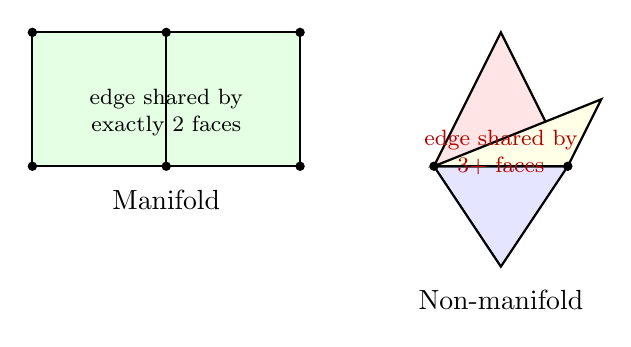
\begin{tikzpicture}[scale=0.85]
  \begin{scope}[xshift=-3cm]
    \draw[thick,fill=green!10] (0,0)--(2,0)--(2,2)--(0,2)--cycle;
    \draw[thick,fill=green!10] (2,0)--(4,0)--(4,2)--(2,2)--cycle;
    \fill (0,0) circle (2pt); \fill (2,0) circle (2pt); \fill (4,0) circle (2pt);
    \fill (0,2) circle (2pt); \fill (2,2) circle (2pt); \fill (4,2) circle (2pt);
    \node at (2,-0.5) {Manifold};
    \node[font=\footnotesize] at (2,1) {edge shared by};
    \node[font=\footnotesize] at (2,0.6) {exactly 2 faces};
  \end{scope}
  \begin{scope}[xshift=3cm]
    \draw[thick,fill=red!10] (0,0)--(2,0)--(1,2)--cycle;
    \draw[thick,fill=blue!10] (0,0)--(2,0)--(1,-1.5)--cycle;
    \draw[thick,fill=yellow!10] (0,0)--(2,0)--(2.5,1)--cycle;
    \fill (0,0) circle (2pt); \fill (2,0) circle (2pt);
    \node at (1,-2) {Non-manifold};
    \node[font=\footnotesize,red!70!black] at (1,0.4) {edge shared by};
    \node[font=\footnotesize,red!70!black] at (1,0) {3+ faces};
  \end{scope}
\end{tikzpicture}
\caption{(Left)~Manifold mesh: every edge is shared by exactly two faces. (Right)~Non-manifold: an edge shared by three faces violates the manifold property.}
\label{fig:manifold}
\end{figure}
